\chapter{Standard reference frame and local parameters}
\label{appendix_1a}
\bibliographystyle{nar}  In   addition  to  the   description  of  RNA
structures  at the  level of  torsion  angles, one  can also  describe
structure  in  terms  of  the  spatial  arrangements  of  adjacent  or
associated bases.  The structural description  of RNA used  here comes
from the program \textsf{3DNA} \cite{lu2003}, which reports three sets
of parameters that define the local arrangements of bases.
\begin{enumerate}
\item Base-pair parameters,
\item Base (base-pair) step parameters,
\item Base (base-pair) local helical parameters.
\end{enumerate}
The bases  or base pairs and  the paramenters are  the quantities that
bring  into coincidence  coordinate frames  on the  two  objects using
ideas from classical mechanics.
%% The first two are based on cartesian coordinates
%% (``objectcentered'', reference frame),
%% whereas the third is referred as helical coordinates
%% (non-object centered)
The first two  sets of parameters are based  on Cartesian coordinates,
whereas the  third set  of helical coordinates,  resembles cylindrical
coordinates and is based on the single rotation that brings coordinate
frames  on   the  two  bases  into   coincidence  (Chasles's  theorem)
\cite{babcock1994}.

\section{Base-pair and base-step parameters}
In  \textsf{3DNA}   one  starts  with   a  Protein  Data   Bank  (PDB) formatted
\cite{berman2000}  file   which  is  usually   based  on  experimental
information\footnote{This is the most common  case but the PDB file is
  sometimes  the result of  theoretical modeling.}   and which  can be
downloaded from the Nucleic Acid Database (NDB) or  PDB. This file contains the experimentally
derived Cartesian  coordinates of  the atoms. With  this experimental
data one  performs a least-squares  fit to a standard  reference frame
\cite{olson2001}. This can be done using the \textsf{octave} script at
\url{http://rutchem.rutgers.edu/\~esguerra/RNA/scripts.html}   as  a
tutorial  example.  The  coordinate origin  which is  embedded  in the
standard  reference frame  is kept  and used  for both  base  and base
pairs.  In  the case of single  unpaired bases, the  program keeps the
origin of one  base of an ideal Watson-Crick  pair.  The definition of
this frame is illustrated in Figure~\ref{fig:standard}

\begin{figure}[htbp]
\centering
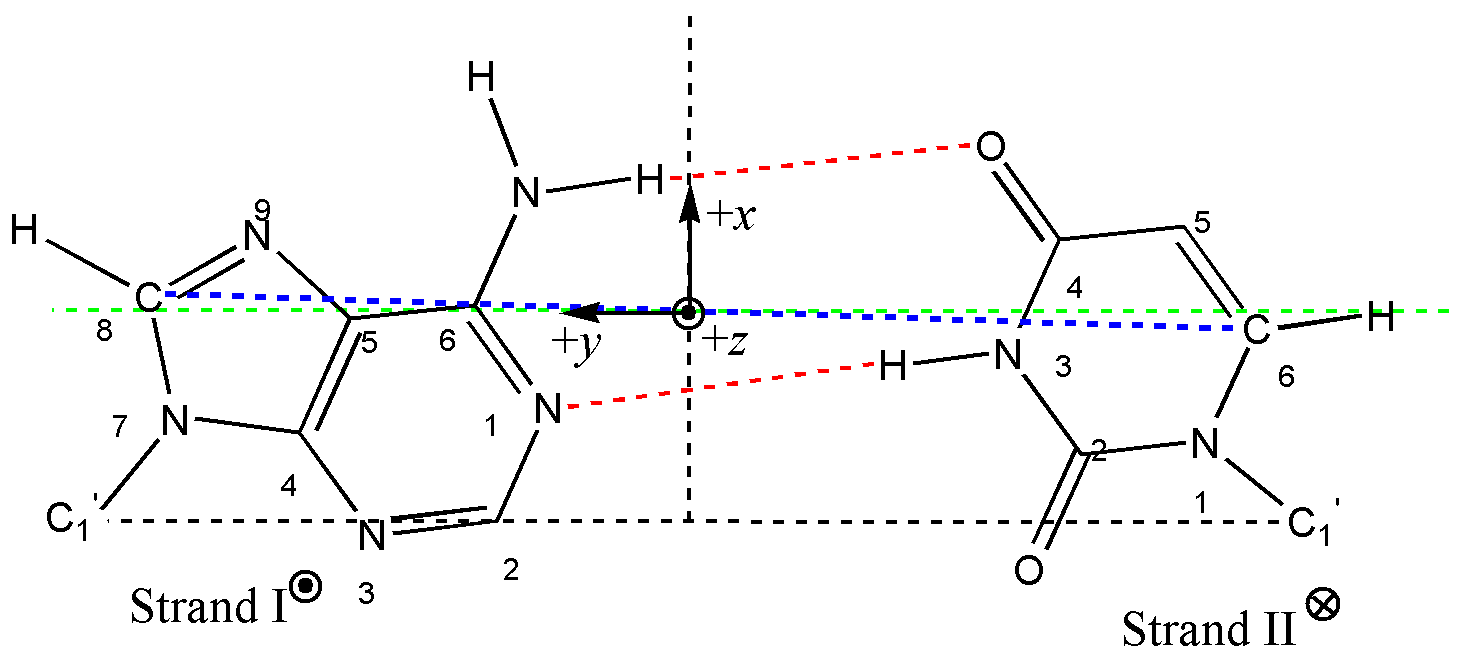
\includegraphics[scale=0.8]{Chapter1/standard.png}
\caption{Standard    reference    frame    of   an    A-T    base-pair
  \cite{olson2001}.  The \textit{y}-axis (dashed green line) is chosen
  to be  parallel to the line  connecting the C1$^{'}$  of adenine and
  the  C1$^{'}$  of  thymine   associated  in  an  ideal  Watson-Crick
  base-pair. The \textit{x}-axis is  the perpendicular bisector of the
  C1$^{'}$  -  C1$^{'}$  line,  and  the  origin  is  located  at  the
  intersection of  the \textit{x}-axis and the line  connecting the C8
  atom of adenine  and the C6 atom of  thymine. The \textit{z}-axis is
  the cross product of the $\hat{x}$ and $\hat{y}$ unit vectors.}
\label{fig:standard}
\end{figure}

Once one has determined the coordinate origins for the two consecutive
bases or base pairs comprising a  step one defines a middle step triad
(MST) \cite{lu1997}. This can be described by the following procedure:

1) Find the angle $\Gamma$ between consecutive normals, \textit{i.e.},
\textit{z}-axis. Since these are unit vectors, the angle is defined by
the dot product:

\begin{gather}
\Gamma = \cos^{-1} (\hat{z}_i \cdot \hat{z}_{i+1})
\end{gather}

2)  Then find the  vector which  is perpendicular  to the  two normals
(\textit{z}-axis). This  vector is obtained from the  cross product of
the  consecutive \textit{z}-axis  (that is,  the normal  to  the plane
formed by the two vectors). This axis is called the roll-tilt axis and
is normalized to form the unit vector $\hat{r_t}$,

\begin{gather}
\hat{r_t} = \frac{\hat{z}_i \times \hat{z}_{i+1}}{|\hat{z}_i \times
\hat{z}_{i+1}|}
\end{gather}

%% Note: Why do you need a matrix? Isn't this always in 3D and therefore
%% just vectors would do? Why the more general matricial way instead of
%% the vectorial representation?
3) To make consecutive \textit{z}  vectors coincide, one uses a linear
homogeneous transformation  $R(\theta)$ about the  roll-tilt axis such
that the original orientation matrices $T_i$ and $T_{i+1}$ are rotated
by $ \theta  = \pm \Gamma / 2$ to yield  the transformed $T_i^{'}$ and
$T_{i+1}^{'}$ orientation matrices.
%% NEED to include GRAPHICS of ANGLES and COORDINATES in general.

\begin{gather}
T_i^{'} = R_{rt}(\pm \Gamma/2) T_{i} \\
T_{i+1}^{'} = R_{rt}(\mp \Gamma/2) T_{i+1}
\end{gather}

The origin  for the middle step  triad is the average  of the position
vectors for the $i$ and $i+1$ reference frames,

\begin{gather}
r_{MST} = \frac{(r_i + r_{i+1})} {2}
\end{gather}

4) Again  using the  dot product  one can find  the angle  between the
transformed  $\hat{y}^{'}$  vectors.   This  angle  is  equal  to  the
magnitude  of   the  Twist  ($\Omega$).    The  dot  product   of  the
$\hat{z}_{MST}$ unit  vector with the vector resulting  from the cross
product of $\hat{y}_{i}^{'}$ and $\hat{y}_{i+1}^{'}$ gives the sign of
$\Omega$. Since  the transformed  \textit{x-y} plane is  orthogonal to
$\hat{z}$ then this applies in the same manner for \textit{x},
%%The  vector resulting  from (yi  X yi+1  has got  to be  parallel or
%%anti-parallel to zMST, there's no other possibility.

\begin{gather}
\Omega = cos^{-1}(\hat{y}_{i}^{'} \cdot \hat{y}_{i+1}^{'})\\
(\hat{y}_{i}^{'} \times \hat{y}_{i+1}^{'}) \cdot \hat{z}_{MST} > 0, \quad \textrm{then} \ \Omega > 0\\
(\hat{y}_{i}^{'} \times \hat{y}_{i+1}^{'}) \cdot \hat{z}_{MST} < 0, \quad \textrm{then} \ \Omega < 0
\end{gather}

%%if normalized beforehand then the rule would be,
%%\begin{gather}
%%(\hat{y}_{i}^{'} \times \hat{y}_{i+1}^{'}) \cdot \hat{z}_{mst} = 1, \quad %%then \ \Omega > 1\\
%%(\hat{y}_{i}^{'} \times \hat{y}_{i+1}^{'}) \cdot \hat{z}_{mst} =
%%-1,\quad then \ \Omega < -1
%%\end{gather}

5) With more scalar product one  can find other angles, such as the phase
angle $\phi$,
%% Show in figure.

\begin{gather}
\phi = cos^{-1}(\hat{rt} \cdot \hat{y}_{MST})\\
(\hat{rt} \times \hat{y}_{MST}) \cdot \hat{z}_{MST} > 0, \quad \textrm{then} \ 180 \geq \phi \geq 0\\
(\hat{rt} \times \hat{y}_{MST}) \cdot \hat{z}_{MST} < 0, \quad \textrm{then} \ -180 \leq \phi \leq 0
\end{gather}

6) The  roll $\rho$  and tilt $\tau$  angles, which are  the remaining
angular degrees of  freedom for step parameters, are  defined in terms
of the bending angle and the phase angle:
%as if we were doing a change of variables from cartesian to polar.

\begin{gather}
\rho = \Gamma cos (\phi)\\
\tau = \Gamma sin (\phi)
\end{gather}

Now to  get the remaining  three translational degrees of  freedom for
step  parameters  ($Dx,  Dy,  Dz$)  one  just  needs  to  express  the
displacement vector in the middle step triad frame:

\begin{gather}
[D_xD_yD_z]=T_{MST}(r_{i+1} - r_{i})
\end{gather}

The  procedure  is  completely  analogous  to  compute  the  base-pair
parameters.   The  opening $\omega$,  buckle  $\kappa$, and  propeller
$\sigma$  are the  analogs of  twist $\Omega$,  roll $\rho$,  and tilt
$\tau$, and  the middle  step triad is  called middle base  triad MBT.
The axis  which are made to  coincide are the  \textit{y}-axis and not
the \textit{z}-axis as in the base-pair step case \cite{lu1997}.

The parameters obtained by  this procedure are depicted graphically in
Figure~\ref{fig:allparam}.
\begin{figure}[htbp]
\centering
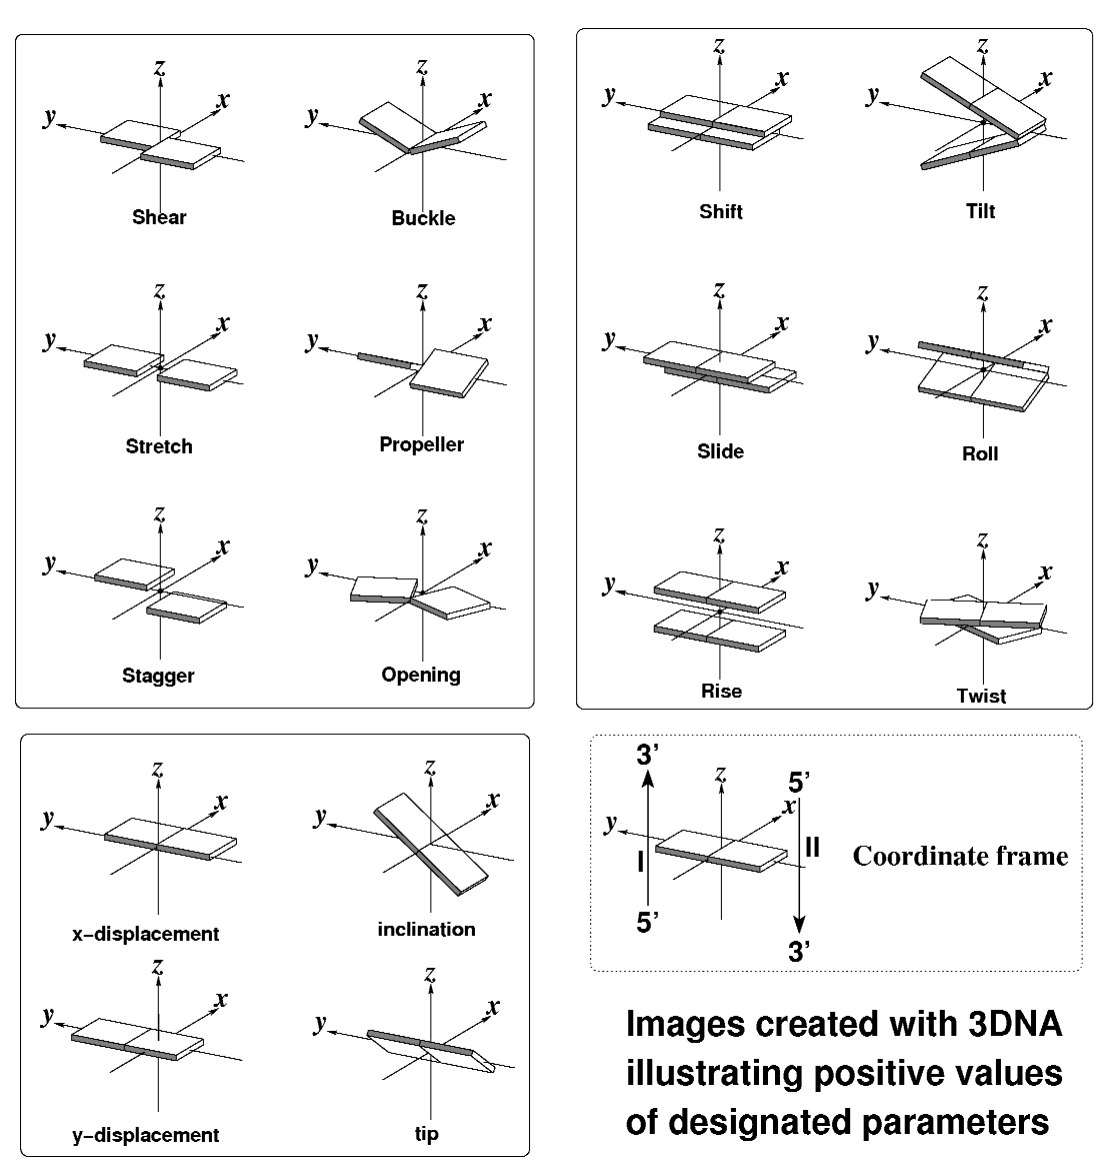
\includegraphics[scale=0.6]{Chapter1/allparam2.png}
\caption{Illustration of base pair and base step parameters \cite{lu2003}}
\label{fig:allparam}
\end{figure}


%\begin{gather}
%\gamma = \cos^{-1} (\hat{y}_{iII} \cdot \hat{y}_{iI})\\
%bo = \hat{y}_{iII} \times \hat{y}_{iI}\\
%\hat{bo} = \frac {bo}{\sqrt{bo \cdot bo}}\\
%T_{iII}^{'} = R_{bo}(+\frac{\gamma}{2}) T_{iII} \\
%_{iI}^{'} = R_{bo}(-\frac{\gamma}{2}) T_{iI}\\
%r_{mbt} = \frac{(r_{iII} + r_{iI})} {2}\\
%\omega = cos^{-1}(\hat{x}_{iII}^{'} \cdot \hat{x}_{iI}^{'})\\
%(\hat{x}_{iII}^{'} \times \hat{x}_{iI}^{'}) \cdot \hat{y}_{MBT} > 0, \quad then \ \omega > 0\\
%(\hat{x}_{iII}^{'} \times \hat{x}_{iI}^{'}) \cdot \hat{y}_{MBT} < 0, \quad then \ \omega < 0\\
%\phi^{'} = cos^{-1}(\hat{bo} \cdot \hat{x}_{MBT})\\
%(\hat{bo} \times \hat{x}_{MBT}) \cdot \hat{y}_{MBT} > 0, \quad then \ 180 \geq \phi^{'} \geq 0\\
%(\hat{bo} \times \hat{x}_{MBT}) \cdot \hat{y}_{MBT} < 0, \quad then \ -180 \leq \phi^{'} \leq 0\\
%\kappa = \gamma cos (\phi^{'})\\
%\sigma = \gamma sin (\phi^{'})\\
%[S_xS_yS_z]=T_{MBT}(r_{iI} - r_{iII})
%\end{gather}

\section{Local helical parameters}

Local helical parameters are determined using Chasles's theorem, which
states \cite{babcock1994}:
\begin{quote}
``\textit{One can  always transport  a free rigid  body from one  position and
  orientation  to  another  position   and  orientation  by  a  single
  continuous motion along a unique axis of rotation.}''
\end{quote}

\noindent For  the three dimensional  case of nucleic acid  base steps
what   this  means   is   that,  instead   of   rotating  around   one
reference-frame  centered  axis  and  then translating  along  another
reference-frame centered  axis, one rotates about  and also translates
along   only   one  common   axis,   which   is  not   reference-frame
centered. This allows one to  define the orientation of a helical axis
(or unique  rotational-translational axis) as  a unit vector  given by
equation 2.15:

\begin{gather}
h=\left[ \begin{array}{c}
h_x\\
h_y\\
h_z
\end{array} \right]
\end{gather}
where:
\begin{gather}
h_x = \frac{\tau}{\Omega_h}, \qquad h_y = \frac{\rho}{\Omega_h},
\qquad h_z = \frac{\Omega}{\Omega_h}
\end{gather}

\begin{gather}
\Omega_h = \sqrt{\tau^2 + \rho^2 + \Omega^2}
\end{gather}

The local helical axis can be defined alternatively \cite{bansal1995}
as a cross product:

\begin{gather}
h = (x_2 - x_1) \times (y_2 - y_1)
\end{gather}
where the  $x$ and $y$ refer to  the reference frames on  base pairs 1
and 2.


\bibliography{biblio}


